% Author: Dawid Weiss (http://www.dawidweiss.com/)
\documentclass[a5paper]{article}
\usepackage{verbatim}

\begin{comment}
:Title: Transparent shadows
:Tags: Transparency, Text and math

An interesting technique for creating text boxes with soft semitransparent shadows.
Can for instance be used to spice up a Beamer presentation. 
The shadows are created by drawing a series of rectangles with varying transparency.

:Author: `Dawid Weiss`_
:Source: The `Latex-beamer-users`_ mailing list

.. _Latex-beamer-users: http://www.nabble.com/Transparent-shadows-under-boxes.-tf3999121.html#a11357827
.. _Dawid Weiss: http://www.dawidweiss.com/
\end{comment}

\usepackage[absolute,overlay]{textpos}
\usepackage{graphicx}
\usepackage{tikz}

%
% Boxed environment with semi-transparent shadow.
%
\newlength{\boxw}
\newlength{\boxh}
\newlength{\shadowsize}
\newlength{\boxroundness}
\newlength{\tmpa}
\newsavebox{\shadowblockbox}

\setlength{\shadowsize}{6pt}
\setlength{\boxroundness}{3pt}

\newenvironment{shadowblock}[1]%
{\begin{lrbox}{\shadowblockbox}\begin{minipage}{#1}}%
{\end{minipage}\end{lrbox}%
\settowidth{\boxw}{\usebox{\shadowblockbox}}%
\settodepth{\tmpa}{\usebox{\shadowblockbox}}%
\settoheight{\boxh}{\usebox{\shadowblockbox}}%
\addtolength{\boxh}{\tmpa}%
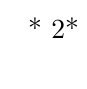
\begin{tikzpicture}
    \addtolength{\boxw}{\boxroundness * 2}
    \addtolength{\boxh}{\boxroundness * 2}

    \foreach \x in {0,.05,...,1}
    {
        \setlength{\tmpa}{\shadowsize * \real{\x}}
        \fill[xshift=\shadowsize - 1pt,yshift=-\shadowsize + 1pt,
                black,opacity=.04,rounded corners=\boxroundness]
            (\tmpa, \tmpa) rectangle +(\boxw - \tmpa - \tmpa,
                \boxh - \tmpa - \tmpa);
    }

    \filldraw[fill=yellow!50, draw=black!50, rounded corners=\boxroundness]
        (0, 0) rectangle (\boxw, \boxh);
    \draw node[xshift=\boxroundness,yshift=\boxroundness,
        inner sep=0pt,outer sep=0pt,anchor=south west]
             (0,0) {\usebox{\shadowblockbox}};
\end{tikzpicture}}

\begin{document}

%
% We prepare a transparent box first.
%
\newsavebox{\mybox}
\begin{lrbox}{\mybox}
\begin{shadowblock}{5cm}
This is a block of text with a transparent
shadow!
\end{shadowblock}
\end{lrbox}

%
% Over existing text
%
Lorem ipsum dolor sit amet, consectetuer adipiscing elit. Phasellus in nunc
tincidunt sapien sodales tincidunt. Nulla posuere semper nunc. Duis lacinia
libero non arcu. Nam quis eros id tortor ultricies fermentum. Aenean vulputate
adipiscing nulla. Etiam fermentum elit ut est. Duis at est at enim imperdiet
vestibulum. In risus dui, malesuada eu, fermentum vel, adipiscing sodales, eros.
Praesent egestas. Aliquam auctor. Maecenas vulputate mollis est. Nam varius. Nam
%auctor fermentum tellus. Curabitur lacus sapien, scelerisque vulputate,
%consectetuer laoreet, fringilla laoreet, tellus. Duis dignissim est non mauris.
%Nam magna velit, pulvinar vel.

\raisebox{2cm}[0pt][0pt]{\makebox[0pt]{\usebox{\mybox}}}


%
% Over a picture.
%
\noindent\includegraphics[width=\linewidth]{img/pipeauv}\\
\hspace*{4cm}\raisebox{1cm}[0pt][0pt]{\makebox[0pt]{\usebox{\mybox}}}


%
% Absolute positioning with textpos
%

\begin{textblock}{4}(2,5.2)
\begin{shadowblock}{4cm}
And a small one on top of it.
\end{shadowblock}
\end{textblock}

\begin{textblock}{4}(0,4.5)
\begin{shadowblock}{4cm}
Absolutely positioned box with a lot of text.
Absolutely positioned box with a lot of text.
Absolutely positioned box with a lot of text.
Absolutely positioned box with a lot of text.
\end{shadowblock}
\end{textblock}

\end{document}

